\section{Speicher}
\label{sec:speicher}

\paragraph{Begriffe}
\begin{items}
	\item \underline{Hauptspeicher}: "`Gedächtnis"' des Rechners. Beinhaltet Programme und Daten, die jederzeit und sofort (\emph{random access}) zur Verfügung stehen müssen
	\begin{figure}[H]\centering\label{Hauptspeicher-Struktur}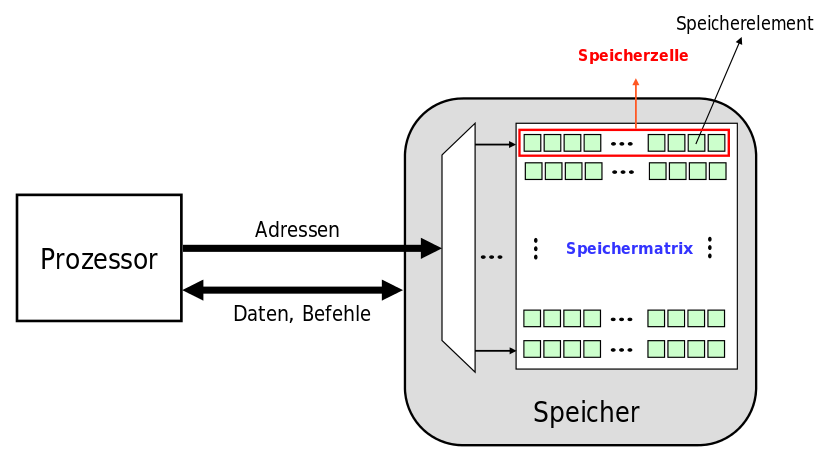
\includegraphics[width=0.33\textwidth]{Hauptspeicher-Struktur}\end{figure}

	\item \underline{Speicherelement}: 1 Bit Speicher

	\item \underline{Speicherzelle}: feste Anzahl von Speicherelementen, auswählbar durch eindeutige Adresse. 8,16,32,\dots Bit

	\item \underline{Speicherwort}: maximale Anzahl an Speicherelementen, die in einem Buszyklus zwischen Mikroprozessor und Speicher übertragen werden können \( \leadsto \) Speicherwortbreite \( = \) \emph{Datenbusbreite}

	\item \underline{Wahlfreier Zugriff}: Jede Speicherzelle kann direkt angesprochen werden (ohne andere Zellen ansprechen zu müssen), Selektion über Adressdecoder

	\item \underline{Speicherorganisation}: Definition über Anzahl \( n \) der Zeilen und Anzahl \( m \) der Speicherelemente pro Zeile, z.B. 16-MBit-DRAM mit Organisation 4Mx4/2Mx8/1Mx16

	\item \underline{Kapazität}: Informationsmenge, die im Speicher untergebracht werden kann (\( n*m \) Bit)

	\item \underline{Arbeitsgeschwindigkeit}:
	\begin{enumeration}
		\item \textbf{Zugriffszeit} (\emph{}access time): maximale Zeit zwischen Anlegen einer Speicheradresse imd Ausgabe der gewünschten Daten

		\item \textbf{Zykluszeit} (\emph{cycle time}): minimale nötige Zeit zwischen zwei hintereinanderfolgenden Adressenaufschaltengen an den Speicher

		\begin{figure}[H]\centering\label{ZykluszeitZugriffszeit}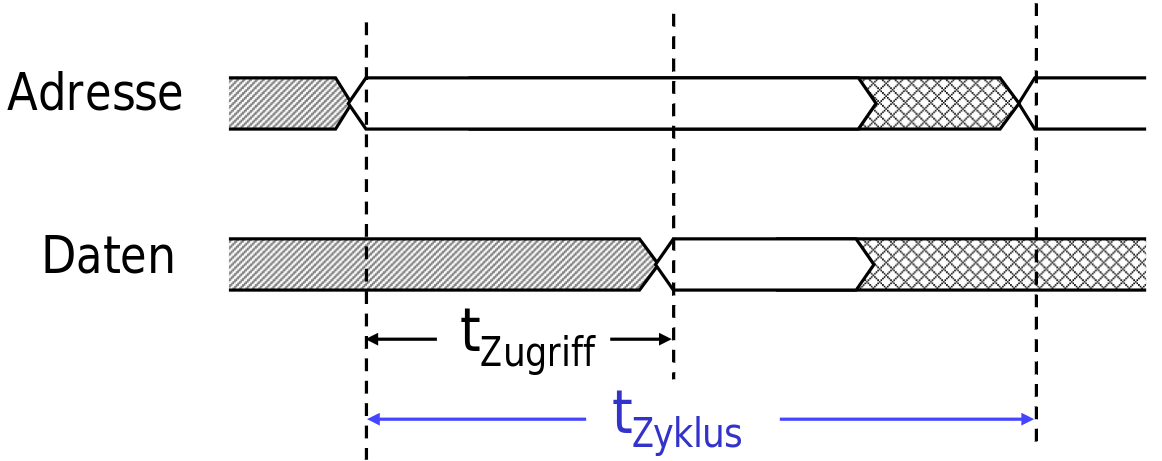
\includegraphics[width=0.33\textwidth]{ZykluszeitZugriffszeit}\end{figure}
	\end{enumeration}
\end{items}

\paragraph{Speicherklassifizierung}
\begin{figure}[H]\centering\label{Speicherklassifizierung}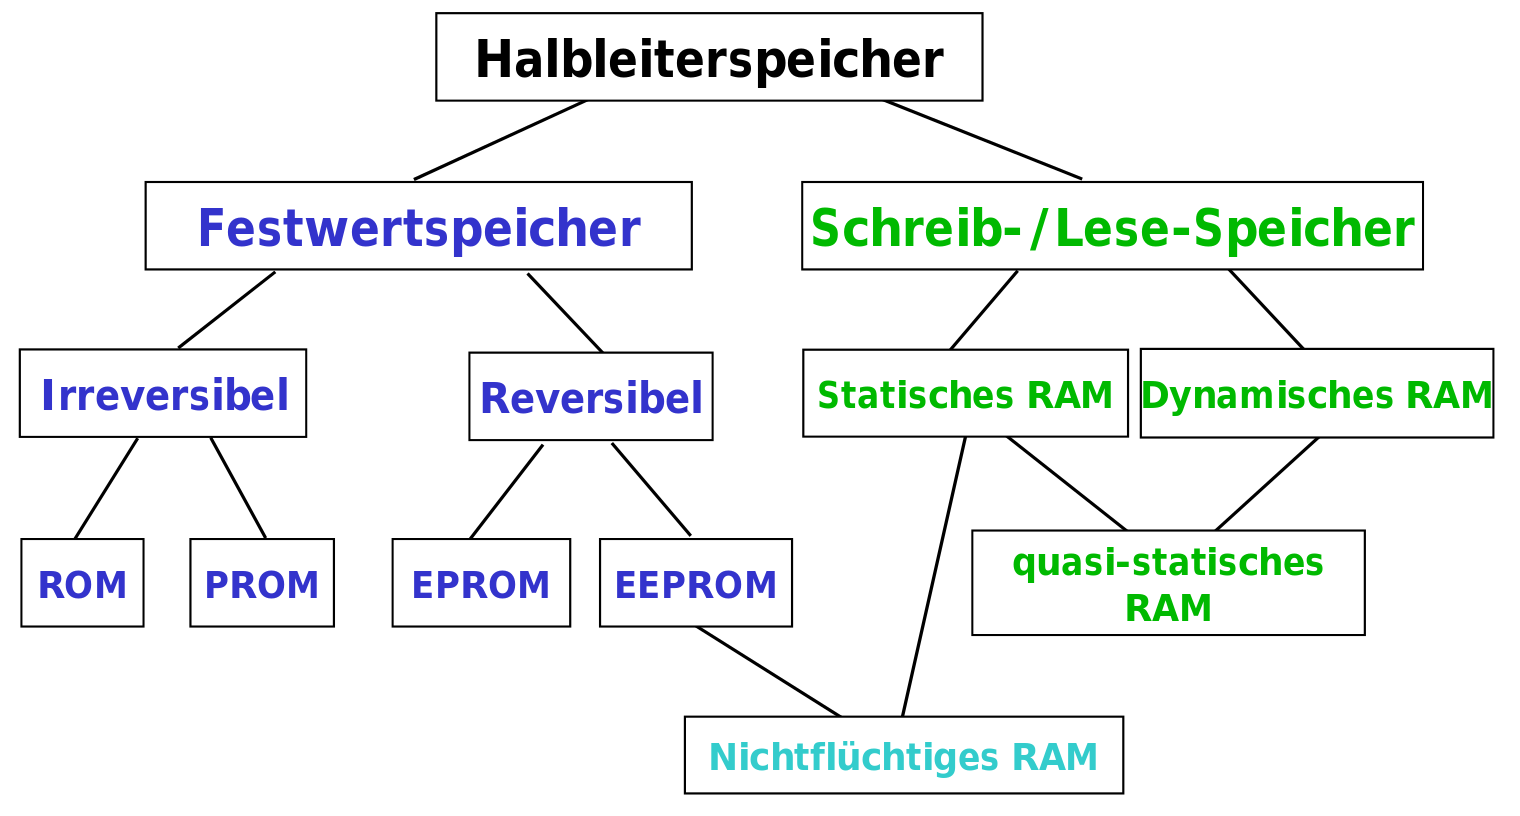
\includegraphics[width=0.33\textwidth]{Speicherklassifizierung}\end{figure}

\newpage

\paragraph{Transistor (MOSFET)}
\begin{items}
	\item Eine Spannung an einem \emph{Gate} regelt, ob Strom zwischen \emph{Source} und \emph{Drain} fließt.
	\item \underline{n-MOS-MOSFET}: Kanal sperrt, wenn keine Spannung anliegt (\emph{selbstsperrend})
\end{items}
\begin{figure}[H]\centering\label{MOSFET}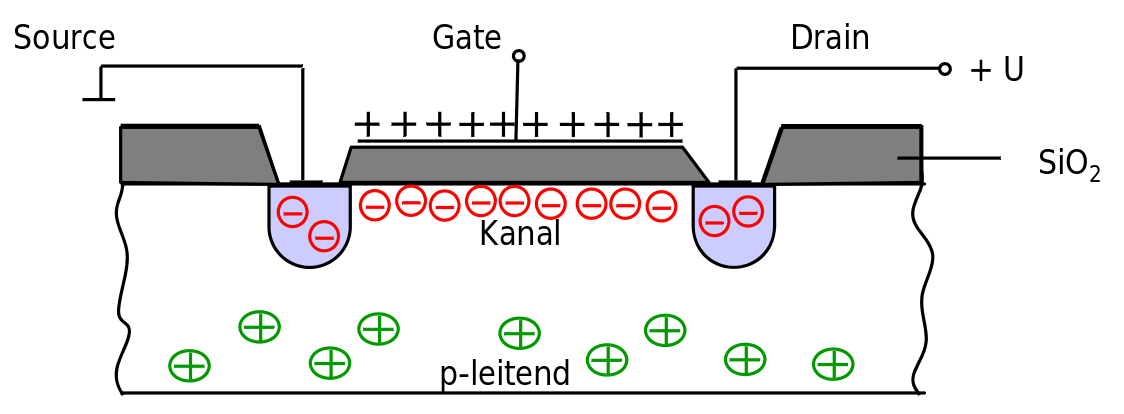
\includegraphics[width=0.33\textwidth]{MOSFET}\end{figure}

\paragraph{Speicherzelle --- statisch (SRAM)}
\begin{items}
	\item Aufgebaut aus zwei kreuzweise rückgekoppelten Invertern und zwei Transistoren zur Ankopplung an Bitleitungen \( \leadsto \) 6-Transistor-Zelle
	\item \underline{Vorteile}: Strom fließt nur zum Umschaltzeitpunkt \( \leadsto \) kein Refresh nötig
	\item \underline{Nachteile}: Hoher Platzverbrauch
\end{items}

\paragraph{Speicherzelle --- dynamisch (DRAM)}
\begin{items}
	\item Aufgebaut aus einer Transistorzelle und einem Kondensator (vergößerte Drain-Zone, von Drain-Kontakt durch dünne Isolierschicht getrennt) \( \leadsto \) Platzverbrauch viermal kleiner als bei SRAM
	\item \underline{Vorteile}: Geringer Platzverbrauch
	\item \underline{Nachteile}: Information geht beim Lesen verloren und muss neu gespeichert werden (\emph{destructive read}), Ladung geht nach einiger Zeit durch Leckströme verloren \( \leadsto \) periodische Auffrischung (\emph{refresh}) nötig
	\item \underline{Lesen}:
	\begin{enumeration}
		\item Leistungskapazität wird vorgeladen (\emph{precharge})
		\item Positive Spannung wird an Gate des Speichertransistors angelegt
		\item Leseverstärker misst Strom am Ende der Bitleitung
	\end{enumeration}
	\item \underline{Schreiben}: 
	\begin{enumeration}
		\item Speichertransistor wird durch Spannung \( U_{GS} \) leitend
		\item Bitleitung auf Masse  \( \leadsto \) Elektronen werden auf Drain-Zone aufgebracht, Kondensator lädt
		\item Bitleitung auf \( U_B \leadsto \) Elektronen von Drain-Zone abgesaugt, Kondensator entlädt 
	\end{enumeration}
\end{items}
\begin{figure}[H]\centering\label{AufbauDRAM}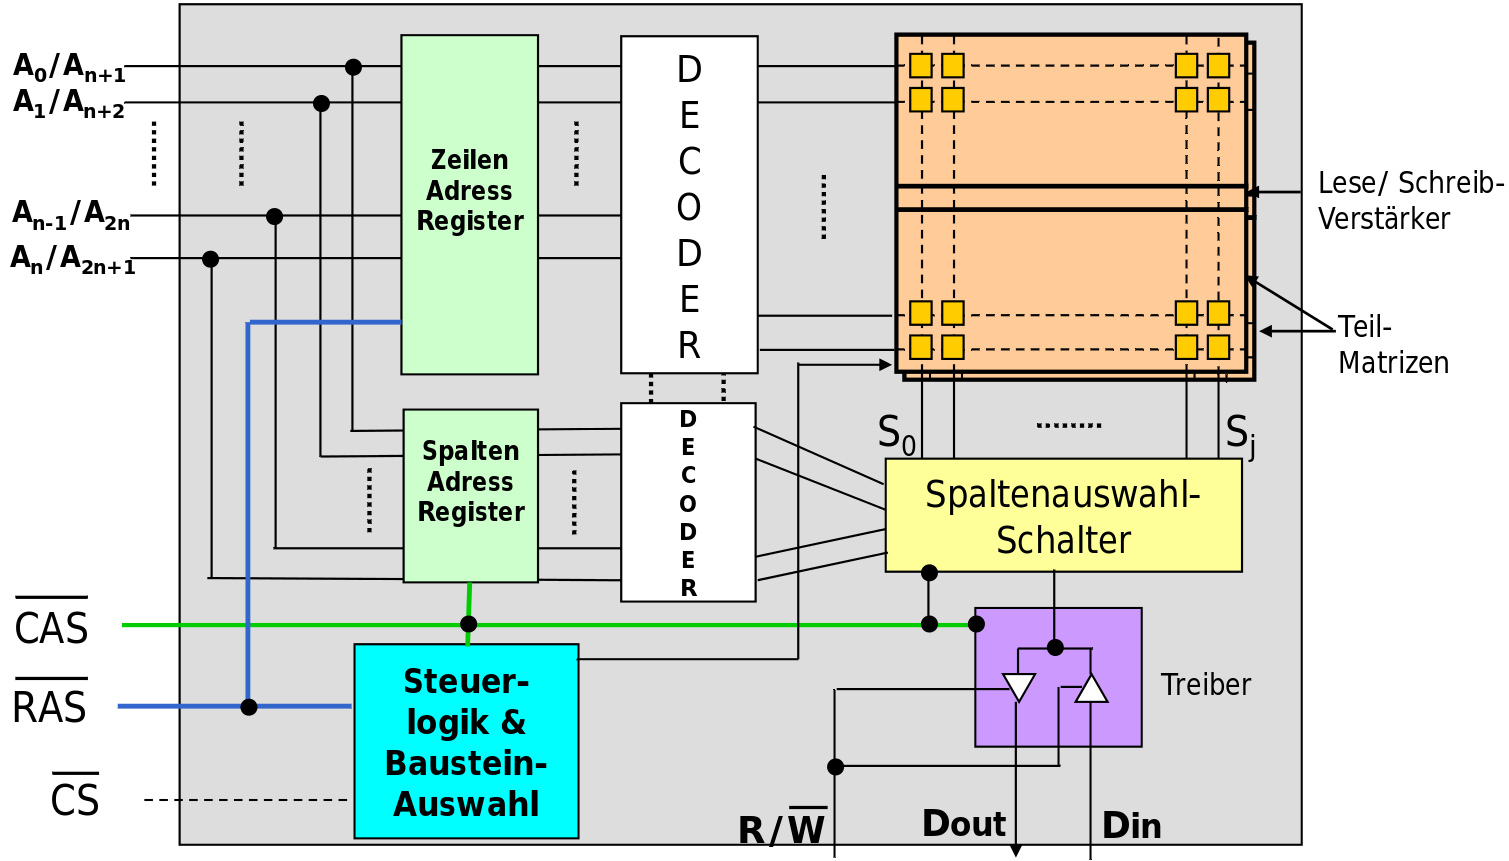
\includegraphics[width=0.5\textwidth]{AufbauDRAM}\end{figure}

\newpage

\paragraph{DRAM --- Adressierung}
\begin{figure}[H]\centering\label{DRAMAdressierung}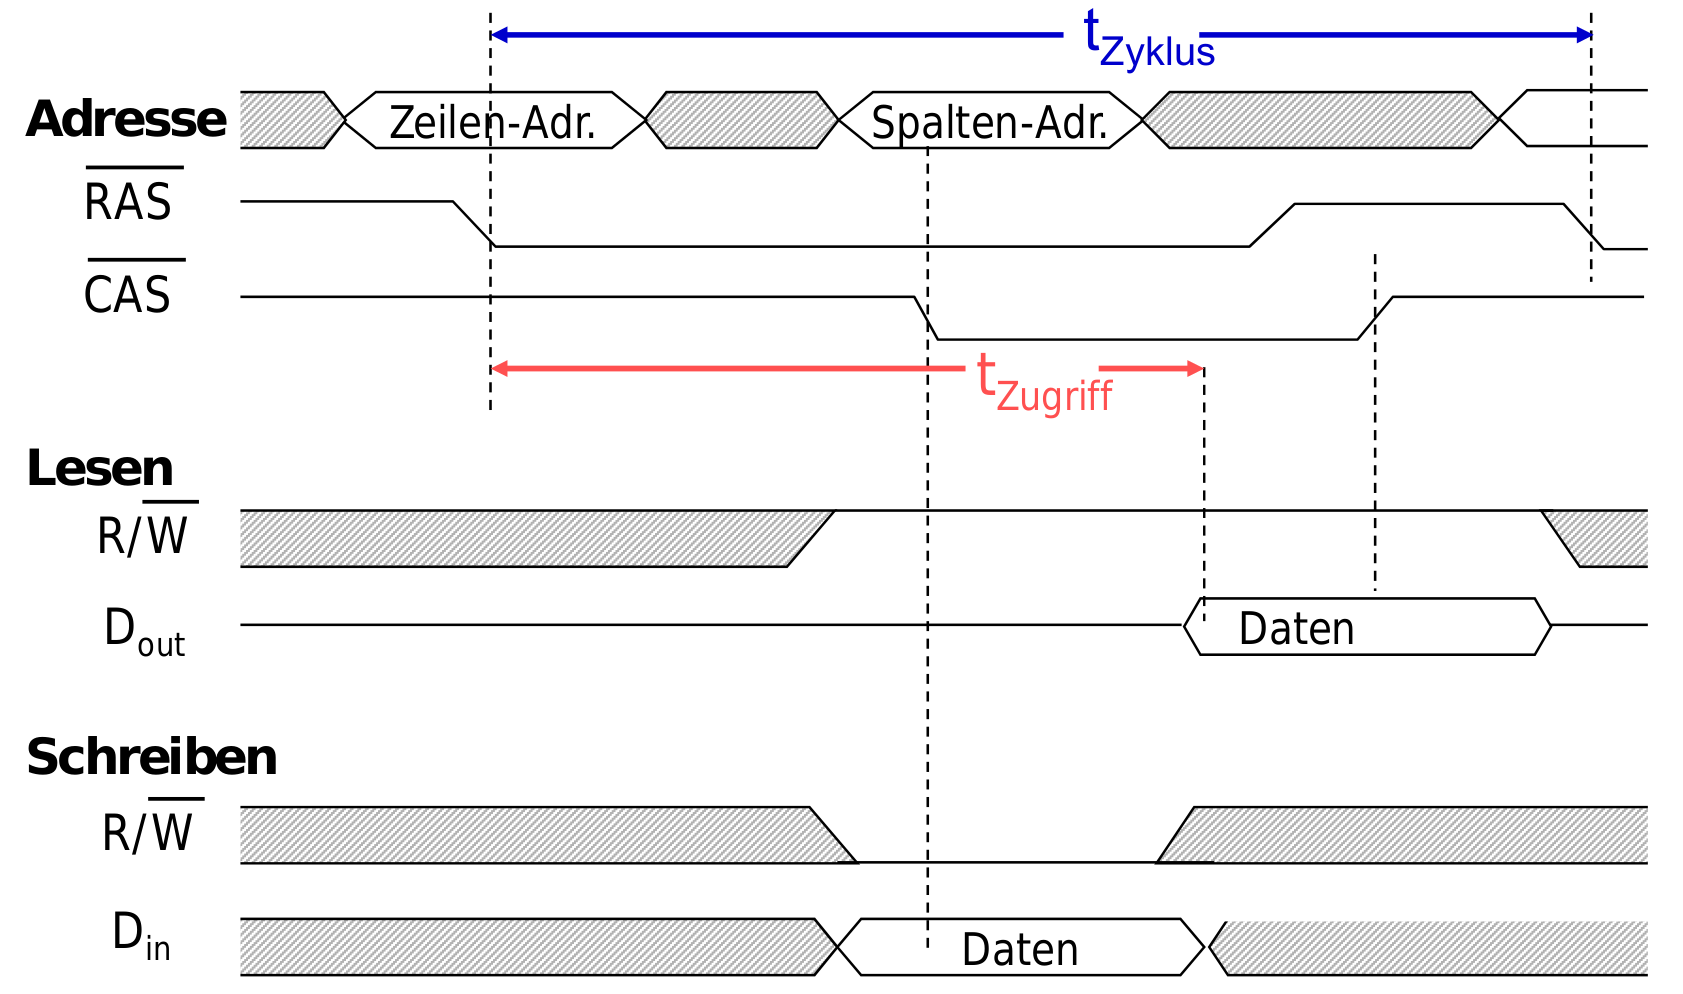
\includegraphics[width=0.33\textwidth]{DRAMAdressierung}\end{figure}

\paragraph{DRAM --- Auffrischung}
\begin{items}
	\item Zeilenweise, jede Zeile alle 2 msec
	\item Nur Zeilenadresse wird an Baustein angelegt, RAS=0, CAS=1
\end{items}

\paragraph{Zugriffsbeschleunigung --- Techniken}
\begin{items}
	\item \underline{Prinzip}: Übertragung von benachbarten Bytes (Blöcken) anstatt einzelnen Bytes \\*
		\( \leadsto \) \textbf{beschleunigter Zugriff} auf Speicherbaustein, falls alle zu \\* \phantom{\( \leadsto \)} lesenden/schreibenden Speicherzellen in einer Zeile liegen \\*
		Zeilenadresse wird auch bei wiederholtem Zugriff auf Zeile (auch \emph{page} genannt) nur einmal angelegt (und im Register gespeichert). Dann werden in schneller Folge die Spaltenadressen angelegt (\emph{fast page mode}: \textbf{FPM-DRAM}) \\*
		\( \leadsto \) \textbf{erheblich beschleunigter Zugriff}
\end{items}

\paragraph{FPM-DRAM}
\begin{items}
	\item aufeinanderfolgende Speicherzugriffe oft in selber Zeile \\*
		 \( \leadsto \) ausnutzen
	\item \underline{Initialisieren}: Wie normaler DRAM
	\item \underline{Nach 1. Lesezyklus}: Speichersteuerung RAS-Signal bleibt aktiv \\*
		\( \leadsto \) Zeile bleibt aktiv
	\item \underline{Bei folgenden Lesezugriffen}: Speichersteuerung übergibt nur noch jeweils eine neue Spaltenadresse an DRAM
	\item \( \leadsto \) RAS-precharche-Zeit und RAS-CAS-Delay entfallen bei Folgezugriffen
\end{items}

\paragraph{EDO-RAM}
\begin{items}
	\item = \emph{extended data output} RAM
	\item Datenausgabe wird bei Lesen von CAS-Signal durch \textbf{interne Pufferung} entkoppelt
	\item \( \leadsto \) Daten stehen länger am Ausgang bereit
	\item \( \leadsto \) bessere Verschachtelungsmöglichkeiten beim Lesen
	\item Prozessor kann Daten auslesen, während Speichersteuerung neue Spaltenadresse an DRAM übergibt
\end{items}

\paragraph{SDRAM}
\begin{items}
	\item = \emph{synchrone dynamische} RAMs
	\item beherrscht heute Speichermarkt
	\item Alle Ein-/Ausgangssignale synchron zum Systemtakt
	\item Prozessor, Chipsatz, Speicher kommunizieren über ein Bussystem (mit einer Frequenz getaktet)
	\item Intern 2 bis 4 Speicherbänke
	\item Nach Anlegen von Zeilen-/Spaltenadresse:
	\begin{enumeration}
		\item Speichersteuerung generiert nachfolgende Adressen
		\item Speichersteuerung führt alternierenden, überlappenden Zugriff auf die Speicherbänke aus
	\end{enumeration}
\end{items}

\paragraph{DDR-SDRAM}
\begin{items}
	\item Nächste Stufe SDRAM (SRAM II)
	\item Vier Speicherbänke, die parallel arbeiten
	\item \underline{Prinzip}: \\*
	 	- Bandbreitenerweiterung durch Nutzung beider Taktflanken \\*
	 	- Daten werden bei steigender + fallender Taktflanke übertragen \\*
	 	\( \leadsto \) doppelter Datendurchsatz
	\item Laufzeitverzögerungen sehr kritisch \\*
		\( \leadsto \) Verwendung von bidirektionalem Strobe-Signal (\textbf{DQS}) zusätzlich zu Systemtakt
\end{items}

\newpage

\paragraph{SLDRAM}
\begin{items}
	\item = \emph{sync link} SDRAM
	\item Weiterentwicklung SDRAM
	\item Höhere erlaubte Busfrequenzen \( \leadsto \) höhere Leistung
\end{items}

\paragraph{Organisation --- Hauptspeicher}
\begin{items}
	\item lineare Liste von Speicherworten
	\item \underline{Aufbau}: Speicherbausteine
	\item \underline{Zugriffszeit}: Abhängig von verwendeten Speicherbausteinen
	\item Breite: IdR Breite des Datenbus
	\item Maximale Kapazität: Gegeben durch Breite des Adressbus
\end{items}

\paragraph{Memory Map}
\begin{items}
	\item = Speicher-Belegungsplan
	\item Gibt an, welche Speicherbausteine auf welchen Bereichen des Hauptspeichers liegen
\end{items}
\begin{figure}[H]\centering\label{MemoryMap}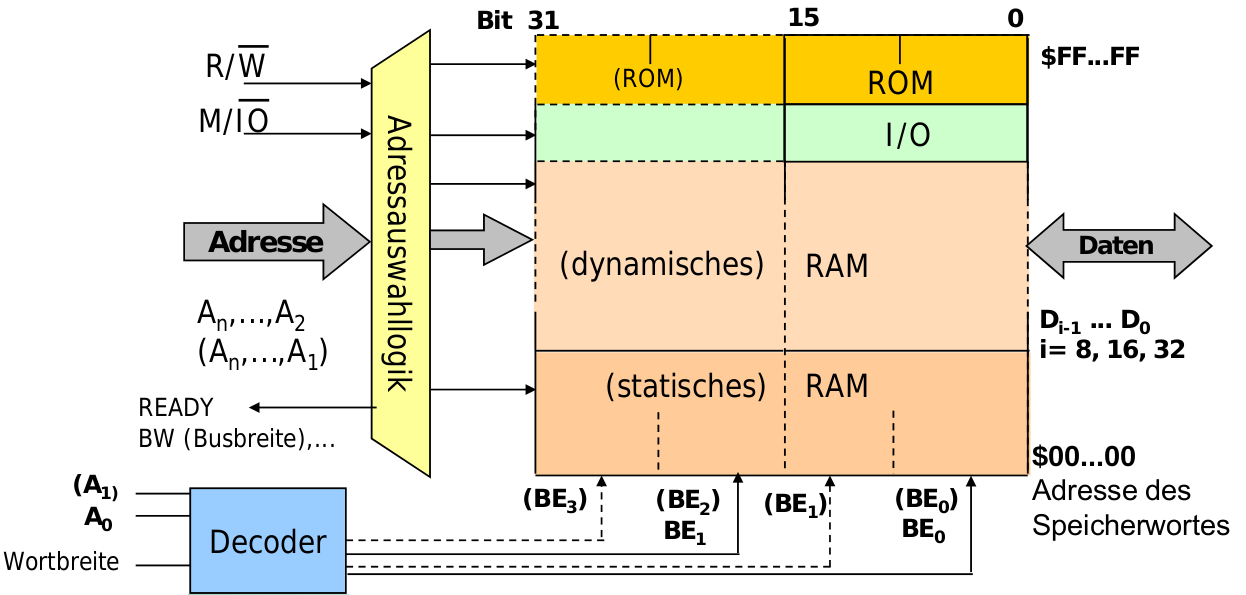
\includegraphics[width=0.33\textwidth]{MemoryMap}\end{figure}